\documentclass[11pt, letterpaper]{article}
\usepackage[utf8]{inputenc}
\usepackage[letterpaper, margin=0.5in]{geometry}
\usepackage{amsmath}
\usepackage{amssymb}
\usepackage{amsthm}
\usepackage{graphicx}
\usepackage{listings}
\usepackage[font=scriptsize]{caption}
\usepackage{subcaption}
\usepackage{xcolor}

\definecolor{codegreen}{rgb}{0,0.6,0}
\definecolor{codegray}{rgb}{0.5,0.5,0.5}
\definecolor{codepurple}{rgb}{0.58,0,0.82}
\definecolor{backcolour}{rgb}{0.95,0.95,0.92}

\lstdefinestyle{mystyle}{
    backgroundcolor=\color{backcolour},   
    commentstyle=\color{codegreen},
    keywordstyle=\color{magenta},
    numberstyle=\tiny\color{codegray},
    stringstyle=\color{codepurple},
    basicstyle=\ttfamily\footnotesize,
    breakatwhitespace=false,
    texcl=true,
    mathescape=true,
    breaklines=true,                 
    captionpos=b,                    
    keepspaces=true,                 
    numbers=left,                    
    numbersep=5pt,                  
    showspaces=false,                
    showstringspaces=false,
    showtabs=false,                  
    tabsize=2
}

\lstset{style=mystyle}
\graphicspath{ {.} }
\captionsetup{justification=raggedright, singlelinecheck=false}

\author{Ryan Tang}
\title{STA 602 HW 9}
\date{November 4th 2022}

\begin{document}
\maketitle

\section{Exercise 7.1}
\paragraph{(a) Jeffrey Prior on the Joint Parameters}
The Jeffrey prior is $p_J(\theta, \Sigma) \propto |\Sigma|^{-(p+2)/2}$. It is not a proper probability density function because it doesn't integrate to 1 and doesn't ensure $\Sigma$ to be positive definite, and symmetric. The only possible way is when the Inverse-Wishart distribution's $\nu_o > p - 1$, where $p$ is the dimension of $X \in \mathbb{R}^p$ in our observations. But the Jeffrey prior implies $\nu_o = 0$, which doesn't guarantee a proper $\Sigma$. Well, we can use it as long as the sample size exceeds the $p-1$ threshold.

\paragraph{(b) Full conditionals}
\begin{align*}
    Y_i &\mathop{\thicksim}^{iid} \mathcal{N}(\theta, \Sigma) && Y_i \in \mathbb{R}^p \\
    p(Y|\theta, \Sigma) &=
        (2\pi)^{-pN/2} |\Sigma|^{-N/2} 
        \exp \left[ -\frac{1}{2} \sum_i^N (y_i-\theta)^{\intercal} \Sigma^{-1} (y_i-\theta) \right] \\
    p_J(\theta, \Sigma) &\propto |\Sigma|^{-(p+2)/2} \\
    p_J(\theta, \Sigma|Y) &\propto p_J(\theta, \Sigma) p(Y|\theta, \Sigma) \\
        &\propto |\Sigma|^{-N/2} |\Sigma|^{-(p+2)/2}
            \exp \left[ -\frac{1}{2} \sum_i^N (y_i-\theta)^{\intercal} \Sigma^{-1} (y_i-\theta) \right] \\
        &\propto |\Sigma|^{-(N+p+2)/2} 
            \exp \left[ -\frac{1}{2} \sum_i^N (y_i-\theta)^{\intercal} \Sigma^{-1} (y_i-\theta) \right] \\ \\
    p_J(\theta|Y, \Sigma) &\propto \exp \left[
            -\frac{1}{2} (\theta^{\intercal}(N\Sigma^{-1})\theta
            + \theta^{\intercal}(N\Sigma^{-1} \bar{y}))
        \right] \\
        &\thicksim \mathcal{N}(\theta|(N\Sigma^{-1})^{-1}N\Sigma^{-1} \bar{Y}, N\Sigma^{-1}) \\ \\
    p_J(\Sigma|Y, \theta) &\propto |\Sigma|^{-(N+p+2)/2} 
            \exp \left[ -\frac{1}{2} \sum_i^N (y_i-\theta)^{\intercal} \Sigma^{-1} (y_i-\theta) \right] \\
        &\propto |\Sigma|^{-(N+1+p+1)/2} \exp \left[ -\frac{1}{2} tr(S \Sigma^{-1}) \right] \\
        &\thicksim \text{inverse-Wishart}(\Sigma | N+1, S) \\
    S &= \sum_i^N (y_i - \theta)^{\intercal} (y_i - \theta)
\end{align*}

\newpage
\section{Exercise 7.2}
\paragraph{(a) Multivariate Normal MLE \& Unit Information Priors}
Here we show that the joint unit information priors consist of two proper conjugate priors for the multivariate Gaussian model. The parameterization of the two priors is just the mean $\bar{y}$ and the unit scatter matrix $\frac{1}{N}S_{\bar{y}}=\frac{1}{N}\sum_i^N(y_i-\bar{y})(y_i-\bar{y})^{\intercal}$ from MLE.
\begin{align*}
    \Lambda &= \Sigma^{-1} \\
    p(X|\theta, \Sigma) &= (2\pi)^{-pN/2} |\Lambda|^{N/2} 
        \exp \left[ -\frac{1}{2} \sum_i^N (y_i-\theta)^{\intercal} \Lambda (y_i-\theta) \right] \\
    \ell(\theta, \Sigma) &= \frac{N}{2} \log |\Lambda| -\frac{1}{2} \sum_i^N (y_i-\theta)^{\intercal} \Lambda (y_i-\theta) \\
    p_U(\theta, \Lambda) &\propto \exp[\frac{1}{N} \ell(\theta, \Lambda)] \\
        &\propto \exp \left[
            \frac{1}{2} \log |\Lambda| -\frac{1}{2N}
            \sum_i^N (y_i-\theta)^{\intercal} \Lambda (y_i-\theta)
        \right] \\
        &\propto |\Lambda|^{\frac{1}{2}} \exp \left[
            -\frac{1}{2N}
            \sum_i^N (y_i-\bar{y}+\bar{y}+\theta)^{\intercal} \Lambda (y_i-\bar{y}+\bar{y}+\theta)
        \right] \\
        &\propto |\Lambda|^{\frac{1}{2}} \exp \left[
            -\frac{1}{2N}
            tr[
                (\sum_i^N(y_i-\bar{y})(y_i-\bar{y})^{\intercal}
                + \sum_i^N(\bar{y}-\theta)(\bar{y}-\theta)^{\intercal}
                + \sum_i^N(y_i-\bar{y})(\bar{y}-\theta)^{\intercal})
                \Lambda
            ]
        \right] \\
        & \quad\quad \sum_i^N(y_i-\bar{y})(\bar{y}-\theta)^{\intercal} = 0 \\
        &\propto |\Lambda|^{\frac{1}{2}} \exp \left[
            -\frac{1}{2}
            tr[
                (\frac{1}{N}\sum_i^N(y_i-\bar{y})(y_i-\bar{y})^{\intercal}
                + \frac{1}{N}\sum_i^N(\bar{y}-\theta)(\bar{y}-\theta)^{\intercal})
                \Lambda
            ]
        \right] \\
        &\propto |\Lambda|^{\frac{1}{2}} \exp \left[
            -\frac{1}{2}
            tr[
                \frac{1}{N}\sum_i^N(y_i-\bar{y})(y_i-\bar{y})^{\intercal} \Lambda
                + (\bar{y}-\theta)(\bar{y}-\theta)^{\intercal} \Lambda
            ]
        \right] \\
        &\propto |\Lambda|^{\frac{1}{2}} \exp \left[
            -\frac{1}{2} tr[\frac{1}{N}S_{\bar{y}}\Lambda] - \frac{1}{2}(\bar{y}-\theta)^{\intercal} \Lambda (\bar{y}-\theta)
        \right] \\
        & \quad\quad \frac{1}{N}S_{\bar{y}} = \frac{1}{N}\sum_i^N(y_i-\bar{y})(y_i-\bar{y})^{\intercal} \\
        &\propto
            |\Lambda|^{\frac{p+1-p-1}{2}} \exp \left[ -\frac{1}{2} tr[\frac{1}{N}S_{\bar{y}}\Lambda] \right]
            |\Lambda|^{\frac{1}{2}} \exp \left[ - \frac{1}{2}(\bar{y}-\theta)^{\intercal} \Lambda (\bar{y}-\theta) \right] \\
        &= Wi(\Lambda|p+1, \frac{1}{N}S_{\bar{y}}) \mathcal{N}(\theta|\bar{y}, \Lambda^{-1}) \\
        &= p(\theta|\Lambda) p(\Lambda) \\ \\
    \theta|\Lambda &\thicksim \mathcal{N}(\bar{y}, \Lambda^{-1}) \\
    \Lambda &\thicksim Wi(p+1, \frac{1}{N}S_{\bar{y}}) \\
\end{align*}

\paragraph{(b) Unit Information Posterior}
If we use MLE's unit information priors, the posterior with the same data happens to be the same form with the effective sample size increased with $N$.
\begin{align*}
    \Lambda &= \Sigma^{-1} \\
    p_U(\theta,\Lambda|Y) &\propto p_U(\Lambda) p_U(\theta|\Lambda) p(Y|\theta, \Lambda) \\
        &\propto
            |\Lambda|^{\frac{p+1-p-1}{2}} \exp \left[ -\frac{1}{2} tr[\frac{1}{N}S_{\bar{y}}\Lambda] \right]
            |\Lambda|^{\frac{1}{2}} \exp \left[ - \frac{1}{2} [
                \theta^{\intercal}\Lambda\theta - \theta^{\intercal}\Lambda\bar{y}]
            \right] \\
            &\quad\,\, \cdot 
            |\Lambda|^{N/2} \exp \left[
                -\frac{1}{2} [tr(S_{\bar{y}}\Lambda) + \theta^{\intercal}N\Lambda\theta - \theta^{\intercal}N\Lambda\bar{y}]
            \right] \\
        &\propto 
            |\Lambda|^{\frac{N+p+1-p-1}{2}} \exp \left[ -\frac{1}{2} tr[\frac{N+1}{N}S_{\bar{y}}\Lambda] \right]
            |\Lambda|^{\frac{1}{2}} \exp \left[ - \frac{1}{2} [
                \theta^{\intercal}(\Lambda+N\Lambda)\theta - \theta^{\intercal}(\Lambda+N\Lambda)\bar{y}
            \right] \\
        &\propto
            Wi(\Lambda | N+p+1, \frac{N+1}{N}S_{\bar{y}})
            \mathcal{N}(\theta | \Sigma_n(\Lambda+N\Lambda)\bar{y}, \Sigma_n = (\Lambda+N\Lambda)^{-1})
\end{align*}

\section{Exercise 7.3}
\paragraph{(a) Posterior}
Since we have known full conditionals, we can directly sample from it using a Gibbs sampler.
\begin{align*}
    \Sigma &\thicksim IW(\nu_o, S_o) \\ 
    \Sigma|Y &\thicksim IW(v_o + n, S_0+S_{\theta}) \\
    S_{\theta} &= \sum_i^N (y_i - \theta)(y_i - \theta)^{\intercal} \\
    \theta &\thicksim \mathcal{N}(\mu_o, \Sigma_o = \Lambda_o^{-1}) \\
    \theta|Y, \Sigma &\thicksim \mathcal{N}(
        \mu_n = \Sigma_n(\Lambda_o\mu_o+N\Lambda\bar{y}),
        \Sigma_n = (\Lambda_o + N\Lambda)^{-1})
    )    
\end{align*}

\paragraph{(b) $\theta$ posteriors}
We can see Blue crabs, on average, generally have smaller body widths and rear widths than orange crabs.
\begin{figure*}[!h]
  \centering
  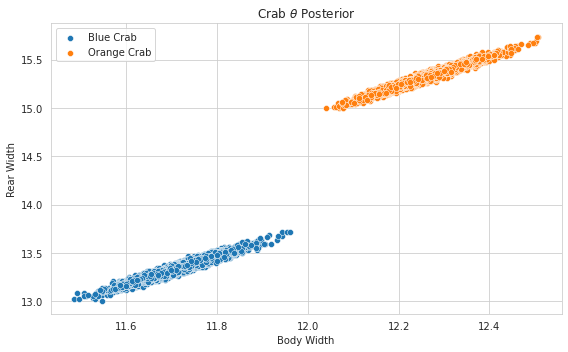
\includegraphics[width=0.5\textwidth]{3.1.png}
  \captionsetup{justification=centering}
  \caption{$\theta$ Posteriors Comparison of two Crabs}
\end{figure*}

\newpage
\paragraph{(c) Correlation on $\Sigma$ posteriors}
Lastly, we plot the posterior correlation between the two crab species. We can see that the Orange crabs' widths are quite consistent between the body and rear widths. The Blue crabs are relatively less consistent. $P[\rho_{blue} < \rho_{orange}|Y] = 0.8299$.
\begin{figure*}[!h]
  \centering
  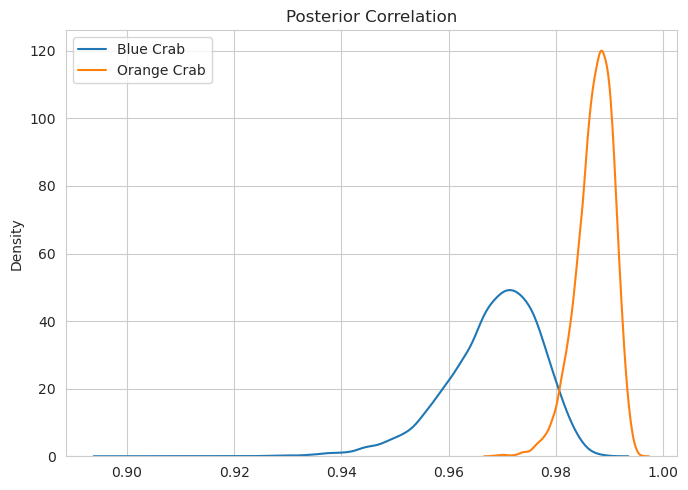
\includegraphics[width=0.5\textwidth]{3.2.png}
  \captionsetup{justification=centering}
  \caption{Correlation Posteriors Comparison of two Crabs. }
\end{figure*}

\paragraph{Appendix}
The code for generating the posterior samples is included here for completeness.
\begin{lstlisting}[language=Python]
import pandas as pd
import numpy as np
import matplotlib.pyplot as plt
import seaborn as sns
import scipy.stats as stats
from numpy.linalg import inv

sns.set_style('whitegrid')

def cov2corr(S):
    return S[0, 1] / np.sqrt(S[0, 0] * S[1, 1])

blue = pd.read_csv("bluecrab.dat", names=["body","rear"], delimiter=" ")
orange = pd.read_csv("orangecrab.dat", names=["body","rear"], delimiter=" ")

burn_ins = 2000
n_epochs = 10000

# prior parameters
mu0 = blue.mean().values
A0 = S0 = blue.cov().values
v0 = 4

# Blue posterior
N = blue.shape[0]
S = blue.cov()

blue_samples = []
for epoch in range(n_epochs + burn_ins):
    v_n = v0 + N
    S_n = S0 + S
    sigma_pos_rv = stats.invwishart(df=v_n, scale=S_n)

    $\Sigma$ = sigma_pos_rv.rvs()
    $\Sigma$_n = inv(inv(A0) + N*inv($\Sigma$))
    $\mu$_n = $\Sigma$_n @ (inv(A0)@mu0 + N*inv($\Sigma$)@blue.mean())

    theta_pos_rv = stats.multivariate_normal($\mu$_n, $\Sigma$_n)
    $\theta$ = theta_pos_rv.rvs()

    if epoch < burn_ins:
        continue 
    else:
        blue_samples.append(($\theta$, $\Sigma$))
    

# Orange posterior
N = orange.shape[0]
S = orange.cov()

orange_samples = []
for epoch in range(n_epochs + burn_ins):
    v_n = v0 + N
    S_n = S0 + S
    sigma_pos_rv = stats.invwishart(df=v_n, scale=S_n)

    $\Sigma$ = sigma_pos_rv.rvs()
    $\Sigma$_n = inv(inv(A0) + N*inv($\Sigma$))
    $\mu$_n = $\Sigma$_n @ (inv(A0)@mu0 + N*inv($\Sigma$)@orange.mean())

    theta_pos_rv = stats.multivariate_normal($\mu$_n, $\Sigma$_n)
    $\theta$ = theta_pos_rv.rvs()

    if epoch < burn_ins:
        continue 
    else:
        orange_samples.append(($\theta$, $\Sigma$))
\end{lstlisting}


\end{document}